\section{Different Settings}
\begin{figure*}[b]

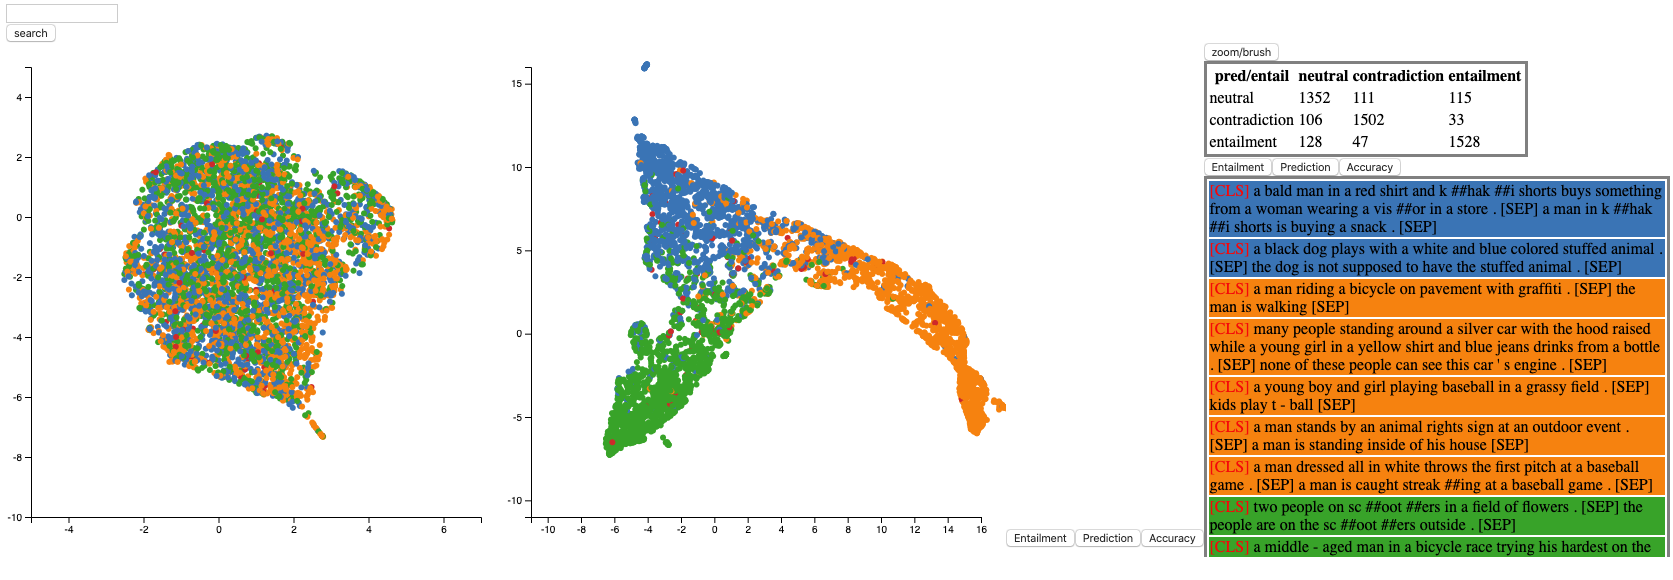
\includegraphics[width=.9\textwidth]{figs/fig6.png}

\caption{Points for only [CLS] tokens}
\label{fig:new1}

\end{figure*}

We also visualize the [CLS] tokens alone using UMAP as shown in fig ~\ref{fig:new1}. So that we can get more sentence level information. And we notice that the observations we found for all tokens still hold for [CLS] tokens. And since [CLS] tokens are more related to the task and the sentences, we can use these plots for debugging purpose. 

\subsection{Debugging}

{\flushleft {\bf (1)}}  
We first check the outlier nodes as shown in fig ~\ref{fig:outliers}. We find that BERT separate the incomplete sentences and sentences with negotiation from other sentences.

{\flushleft {\bf (2)}}  
We then check the sentences which we predicted incorrectly. We find that the error in boundary area is easier for us to correct compared to the error in other area. Like the example we showed in fig ~\ref{fig:false}. We can easily tell that the left example is an entailment, but since our model doesn't learn that saxophone is an instrument, it predict this as a contradiction. But in right-hand side sentences, we get confused as human by the term "his picture", does it mean the picture of himself, or the picture that he takes?

According to this findings, we think we can use this tool for debugging purposes. For some errors in boundary area, we think we can solve them by introducing BERT-large and some knowledge base.


\begin{figure*}[h]

\centering
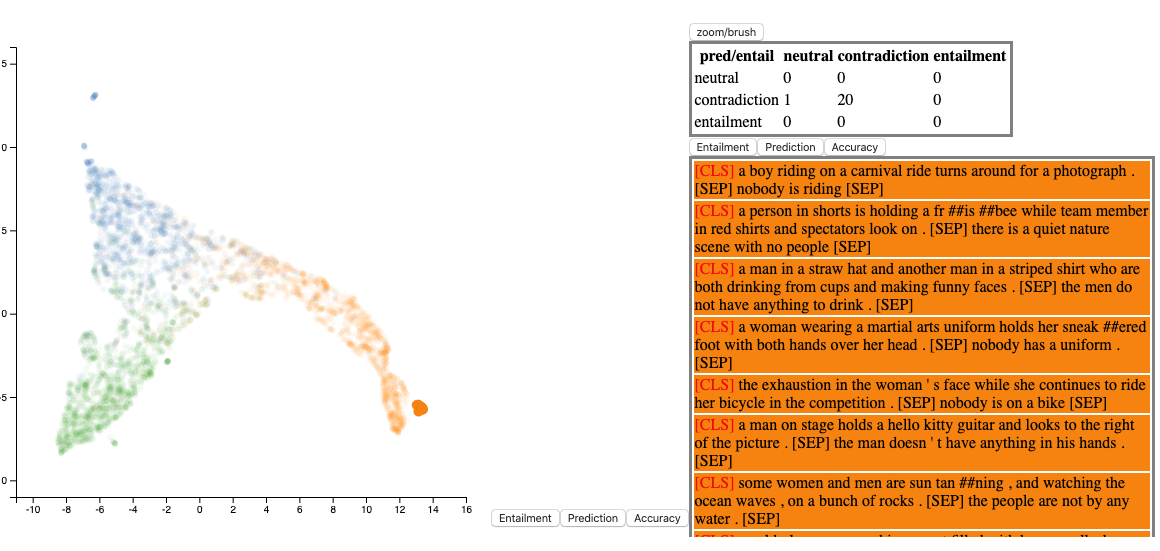
\includegraphics[width=.3\textwidth]{figs/fig8.png}\hfill
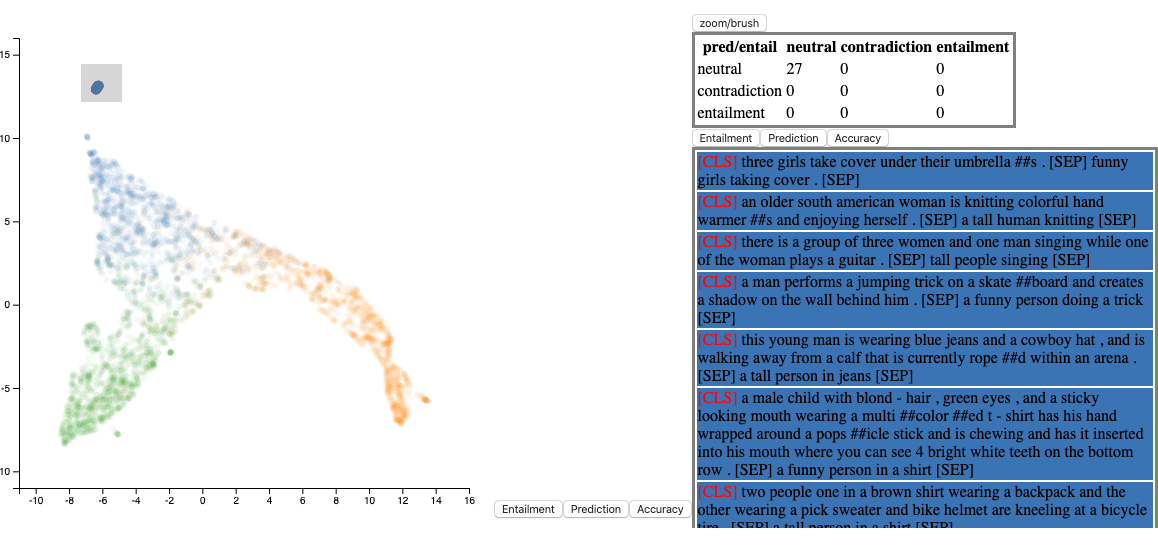
\includegraphics[width=.3\textwidth]{figs/fig9.png}\hfill
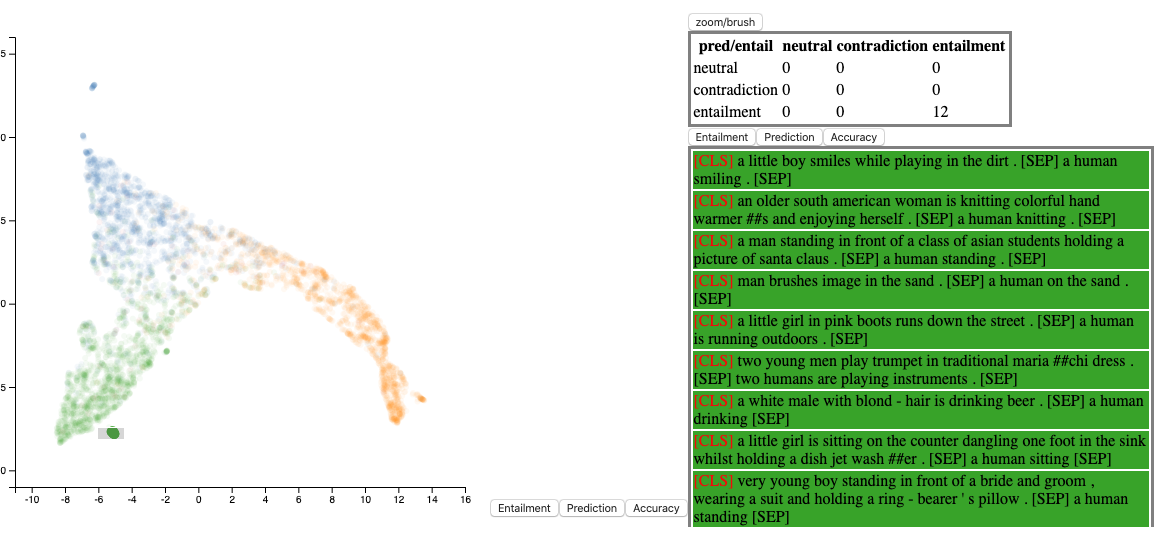
\includegraphics[width=.3\textwidth]{figs/fig10.png}

\caption{Outlier Analysis}
\label{fig:outliers}

\end{figure*}

\begin{figure*}[h]

\centering
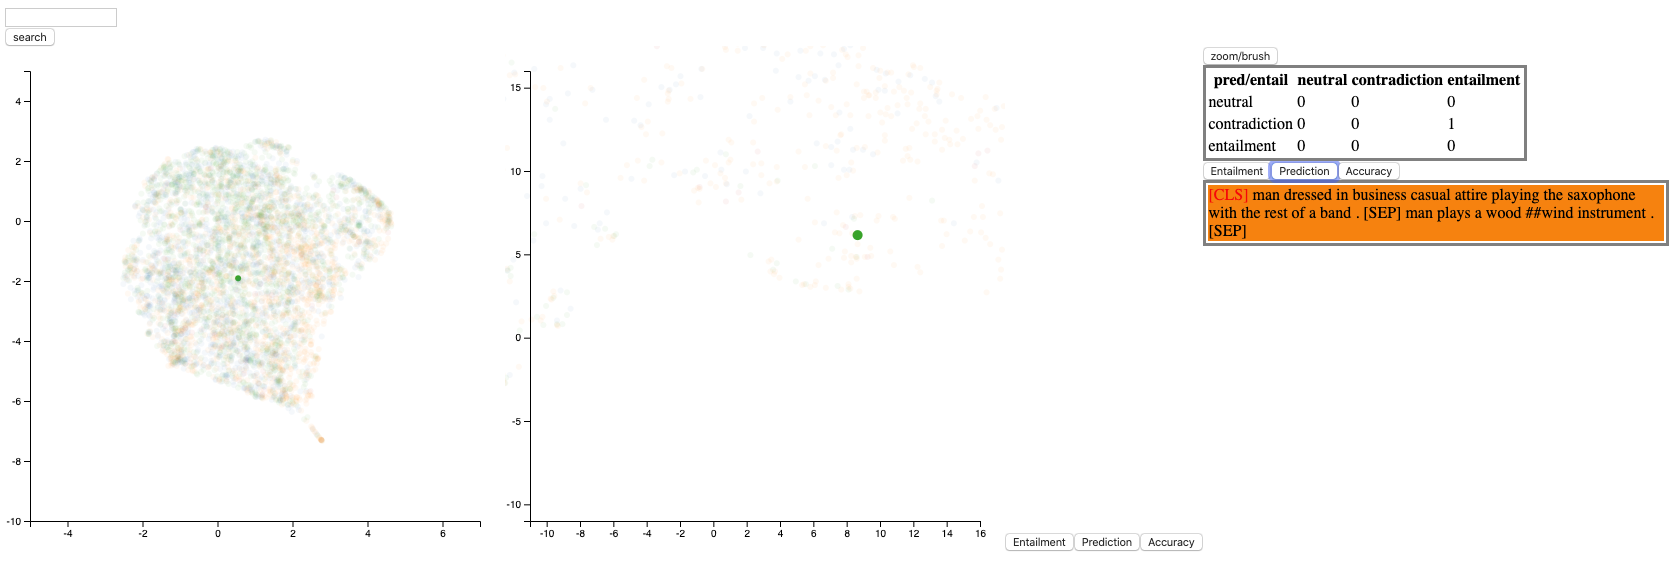
\includegraphics[width=.4\textwidth]{figs/fig7.png}\hfill
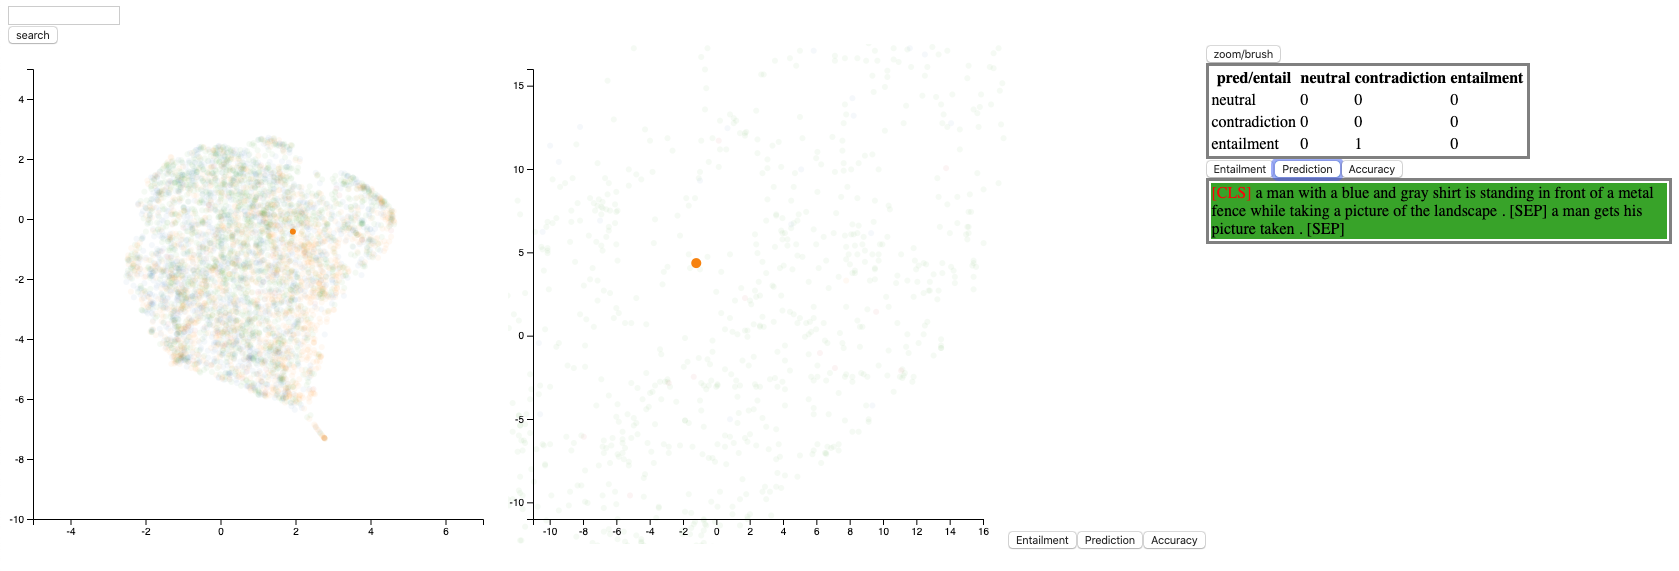
\includegraphics[width=.4\textwidth]{figs/fig11.png}

\caption{Error Analysis}
\label{fig:false}

\end{figure*}
